\documentclass{article}
\usepackage[utf8]{inputenc}
\usepackage{polski}
\usepackage{amsmath,amssymb,graphicx,subfig,pdfpages,enumitem,empheq,verbatim}

\author{Krystian Baran 145000}
\title{Laboratoria zestaw 4}

\begin{document}

\maketitle
\newpage

\section{Przykład projektu zaliczeniowego cz 1}
Długość $X$ (w [mm]) detalu produkowanego na pewnym automacie jest zmienną losową o gęstości prawdopodobieństwa
$$f_{X}(x) = \frac{1}{\sigma\sqrt{2\pi}}\exp\Big(\frac{-x^2+40x-400}{0.08}\Big), x\in\mathbb{R}$$

\begin{enumerate}
\item Rozpoznać rozkład długości detalu i jego parametry, wyznaczyć drugi moment zwykły długości detalu, sporządzić krzywą gęstości i dystrybuantę.
\item Obliczyć prawd. zdarzeń: $|X-19.98|\geq 0.02$, $|X-\mathbb{E}X|<\mathbb{D}X$.
\item Dla jakiej wartości stałej $b$ zachodzi równość $P(x_{0.05}<X<b)=0.90$?
\item Wyznaczyć kwartyle długości detalu oraz obliczyć wartości gęstości dla nich.
\item Wyznaczyć przedział, w którym mieści się 95\% produkowanych detali po złomowaniu 5\% detali o największej odchyłce długości od wymiaru przeciętnego.
\item Co wynika z faktu, że łączna długość 180 wyprodukowanych detali będzie mniejsza od 358[cm]?
\item Detal spełnia normę długości, jeśli jego długość mieści się w dopuszczalnym przedziale (19,6; 20,4) [mm]. W celu sprawdzenia dokładności produkcji zmierzona zostanie długość 180 losowo wybranych detali.
\begin{enumerate}
\item Wprowadzić zmienną losową opisującą wynik sprawdzania normy długości badanej partii detali. Podać jej rozkład i sporządzić wykresy PMF i CDF.
\item Obliczyć prawd. zdarzenia, że w badanej partii detali, co najmniej 175 z nich spełni normę długości.
\item Wyznaczyć wartość oczekiwaną, odchylenie standardowe oraz modę liczby detali, które spełnią normę długości i prawdopodobieństwo dla mody.
\end{enumerate}
\end{enumerate}

\subsection*{1}
Korzystając z przekształceń funkcję gęstości sprowadza się to funkcji gęstości rozkładu normalnego z parametrami $\mu$ i $\sigma$.
$$\frac{1}{\sigma\sqrt{2\pi}}\exp\Big(\frac{-x^2+40x-400}{0.08}\Big) = \frac{1}{\sigma\sqrt{2\pi}}\exp\Big(-\frac{(x-20)^2}{2\cdot(0.2)^2}\Big)$$
$$N(\mu,\sigma) = \frac{1}{\sigma\sqrt{2\pi}}\exp\Big(-\frac{(x-\mu)^2}{2\cdot\sigma^2}\Big)$$
Zatem $\mu = 20$ i $\sigma = 0.2$.

\subsection*{2}
Dla $|X-19.98|\geq 0.02$:
\begin{align*}
P(|X-19.98|\geq0.02) & = 1 - P(|X-10.98|<0.02) \\
& = 1 - P(-0.02<X-19.98<0.02) \\
& = 1 - P(19.96<X<20) \\
& = 1 - F_{N(20,0.2)}(20) + F_{N(20,0.2)}(19.96) \\
& \overset{R}{=} 1 - pnorm(20,20,0.2) + pnorm(19.96,20,0.2) \\
& \approx 1 - 0.5 + 0.4207403 \approx 0.9207403
\end{align*}
Gdzie $pnorm(x,\mu,\sigma)$ to funkcja z R obliczająca wartość dystrybuanty rozkładu normalnego dla danego $x$ i z danymi parametrami $\mu$ i $\sigma$.
\\
\par
Dla $|X-\mathbb{E}X|<\mathbb{D}X$ wiemy że $\mu = \mathbb{E}X$ i że $\sigma = \mathbb{D}X$. Zatem:
\begin{align*}
P(|X-\mathbb{E}X|<\mathbb{D}X) & = P(|X-20|<0.2) = P(-0.2<X-20<0.2) \\
& = P(19.8<X<20.2) \\
& = F_{N(20,0.2)}(20.2) - F_{N(20,0.2)}(19.8) \\
& \overset{R}{=} pnorm(20.2,20,0.2) - pnorm(19.8,20,0.2) \\
& \approx 0.8413447 - 0.1586553 \approx 0.6826894
\end{align*}
Gdzie $pnorm()$ to ta sama funkcja co wcześniej. \\
Zatem $P(|X-19.98|\geq0.02) = 0.92$ a $P(|X-\mathbb{E}X|<\mathbb{D}X) = 0.68$.

\subsection*{3}
Dowolny kwantyl rozkładu normalnego wyznacza się za pomocy standardowego rozkładu normalnego, to znaczy:
$$x_{p} = \mu + \sigma\Phi^{-1}(p)$$
Zatem, podstawiając $Z = \frac{X-20}{0.2} \sim N(0,1)$
\begin{align*}
P(x_{0.05}<X<b) & = P\Big(\frac{x_{0.05}-20}{0.2}<\frac{X-20}{0.2}<\frac{b-20}{0.2}\Big) \\
& =  \Phi\Big(\frac{b-20}{0.2}\Big) - \Phi\Big(\frac{x_{0.05}-20}{0.2}\Big) \\
& =  \Phi\Big(\frac{b-20}{0.2}\Big) - \Phi\Big(\frac{20+0.2\cdot\Phi^{-1}(0.05)-20}{0.2}\Big) \\
& =  \Phi\Big(\frac{b-20}{0.2}\Big) - 0.05 = 0.9
\end{align*}
$$ \Phi\Big(\frac{b-20}{0.2}\Big) = 0.95$$
$$\frac{b-20}{0.2} = \Phi^{-1}(0.95)$$
$$b = 20 + 0.2\cdot\Phi^{-1}(0.95) = x_{0.95}$$

\subsection*{4}
Kwartyle wyznaczamy za pomocą funkcji z R $qnorm(p,\mu,\sigma)$ która oblicza wartość kwartyla $p$ dla podanych $\mu$ i $\sigma$.
\begin{align*}
x_{0.25} & = qnorm(0.25,20,0.2) = 19.8651 \\
x_{0.5} & = qnorm(0.5,20,0.2) = 20 \\
x_{0.75} & = qnorm(0.75,20,0.2) = 20.1349
\end{align*}
\\
Wartości gęstości w tych punktach są następujące:
$$f_{N(20,0.2)}(19.8651) = dnorm(19.8651,20,0.2) = 1.588872$$
$$f_{N(20,0.2)}(20) = dnorm(20,20,0.2) = 1.994711$$
$$f_{N(20,0.2)}(20.1349) = dnorm(20.1349,20,0.2) = 1.588872$$
Gdzie $dnorm(x,\mu,\sigma)$ to funkcja Z R obliczająca wartość funkcji gęstości w danym $x$ i danymi parametrami $\mu$ i $\sigma$.

\subsection*{5}
Nie rozwiązane.

\subsection*{6}
Nie rozwiązane.

\subsection*{7}
Załóżmy ze każdy detal produkowany jest niezależnie; wtedy prawdopodobieństwo wyprodukowania $k$ detali 
które mieszczą się w przedziale będzie miało rozkład dwumianowy z parametrami $n = 180$ i $p = P(19.6<X<20.4)$.
\[
	P(Y=k) = \binom{180}{k}p^k\cdot(1-p)^{180-k}, k=0,1,2\dots.
\]
Jako pierwsze trzeba obliczyć p. 
\begin{align*}
p & = P(19.6<X<20.4) \\
& = F_{N(20,0.2)}(20.4) - F_{N(20,0.2)}(19.6)  \\
& \overset{R}{=} pnorm(20.4,20,0.2) - pnorm(19.6,20,0.2)  \\
& \approx 0.9772499 - 0.02275013 \approx 0.9544997
\end{align*}
Zatem $p = 0.95$. 
Wykres gęstości i dystrybuanty zostały sporządzone w R i wyglądają następująco:
\newpage
\begin{figure}[h!]
\begin{center}
\includegraphics[height=0.4\textheight, angle=0]{"lab4zad1_d.png"}
\caption{Gęstość}
\end{center}
\end{figure}

\begin{figure}[h!]
\begin{center}
\includegraphics[height=0.4\textheight, angle=0]{"lab4zad1_f.png"}
\caption{Dystrybuanta}
\end{center}
\end{figure}

\newpage
Prawdopodobieństwo, że co najmniej 175 detali spełni normę jest następujące:
\begin{align*}
	P(Y\geq175) & = 1 - P(Y<175) \\
	& \overset{R}{=} 1 - pbinom(175,180,0.95) \\
	& \approx 1 - 0.9492507 \approx 0.05074934
\end{align*} \\
Zatem prawdopodobieństwo wykonania, co najmniej 175 detali według normy wynosi 0.05.
\par
Wartość oczekiwana zmiennej losowej Y wynosi:
$$\mathbb{E}Y = n\cdot p = 180\cdot0.95 = 171$$
\par
Variancja zmiennej losowej Y wynosi:
$$\mathbb{D}^2(Y) = n\cdot p\cdot(1-p) = 180\cdot 0.95\cdot0.05 = 85.5$$
\par
Odchylenie standardowe zmiennej losowej Y wynosi:
$$\mathbb{D}Y = \sqrt{85.5} \approx 9.2466$$
\par
Aby obliczyć wartość modalną sprawdzimy warunek: $(n+1)p = 181\cdot 0.95 = 171.95$. 
Jest to liczba rzeczywista, zatem wartość modalna wynosi 171.
\par
Prawdopodobieństwo, że wyprodukujemy dokładne wartość modalna odcinków spełniających normę wynosi:
$$P(Y=171) = dbinom(171,180,0.85) = 0.1351751$$
Gdzie $dbinom(k,n,p)$ to funkcja z R obliczająca wartość gęstości dla danego $k$ i danych parametrów $n$ i $p$.

\newpage
\section{Zadanie 2}
Z partii produkowanych wyrobów, wśród których jest 10\% extra, pobierzemy próbę o liczności $n=12$, w celu sprawdzenia frakcji wyrobów extra w próbie.
\begin{enumerate}[label = \alph*)]
\item Jaki jest rozkład liczby wyrobów extra w próbie, tj. zm. l. $T_n$?
\item Czy rozsądne jest aproksymowanie zm. l. $T_n$ rozkładem normalnym?
\item Obliczyć prawd. zdarzenia $T_n \geq 2$.
\item Obliczyć wartości oczekiwane i wariancje zm. losowych $T_n$ i $P_n$.
\end{enumerate}

\subsection*{a)}
Rozkład liczby wyrobów extra można przybliżyć rozkładem hipergeometrycznym z parametrami $N$ i $K=\frac{N\cdot10}{100}$.
\[
P(X=k) \sim \frac{\binom{N}{K}\binom{N-K}{12-k}}{\binom{N}{12}}
\]

\subsection*{b)}
Jeżeli $X \sim Hypergeom(N,K,n)$, $p=\frac{K}{N}$ i $N$ jest dostatecznie dużą liczbą, wtedy:
\[
P(X\leq k) \approx \Phi\Big( \frac{k-np}{\sqrt{np(1-p)}}\Big)
\]
Zatem możemy przybliżyć rozkład prawdopodobieństwa do rozkładu normalnego.

\subsection*{c)}
Korzystając z aproksymacji z podpunktu \textbf{b} obliczamy wartość $p=\frac{K}{N}=\frac{N}{10N}=0.1$. Wtedy $P(X\geq2)$ wynosi:
\begin{align*}
P(X\geq2) & = 1 - P(X<2) \approx 1 - \Phi\Big( \frac{2-12\cdot0.1}{\sqrt{12\cdot0.1(0.9)}} \Big) \\ 
& \approx 1 - \Phi\Big( \frac{0.8}{1.03923}\Big) \approx 1 - \Phi(0.769800) \\
& \approx 1 - \Phi(0.77) \approx 1 - 0.7794 \approx 0.2206
\end{align*}
Zatem prawdopodobieństwo wynosi 0.22.

\subsection*{d)}
Korzystając z gotowych wzorów na wartość oczekiwaną i wariancję rozkładu hipergeometrycznego otrzymujemy:
\[
\mathbb{E}X = n\frac{K}{N} = 12\cdot0.1 = 1.2
\]
\begin{align*}
\mathbb{D}^2(X) & = n\frac{K}{N} \cdot \frac{N-K}{N} \cdot \frac{N-n}{N-1} \\
& = 1.2\cdot \frac{N\cdot0.9}{N} \cdot \frac{N-12}{N-1} \\
& = 1.08 \cdot \Big( 1 -\frac{11}{N-1}\Big) \\
& = 1.08 -\frac{11.08}{N-1}
\end{align*}
Zatem wartość oczekiwana nie jest zależna od liczby N, natomiast wariancja jest od niej zależna. Aby wariancja nie była wartością ujemną zakłada się, że liczba $N\geq12$, ponieważ nie możemy wziąć więcej wyrobów niż ich jest.

\newpage
\section{Zadanie 3}
Przypuśćmy, że w pewnej populacji ludzi wysokość kobiety: $X\sim N(168;5)$ [cm], a mężczyzny: $Y\sim N(187;7)$ [cm]. Z populacji tej wylosowani zostaną jedna kobieta i jeden mężczyzna. Obliczyć prawd., że
\begin{enumerate}[label=\alph*)]
\item mężczyzna będzie wyższy od kobiety o ponad 10[cm];
\item kobieta będzie wyższa od mężczyzny.
\item średnia arytmetyczna ich wysokości będzie w przedziale (170; 175) [cm].
\item niższa z wylosowanych osób będzie niższa niż 160[cm].
\item wyższa z wylosowanych osób będzie wyższa niż 180[cm].
\end{enumerate}

\subsection*{a)}
Prawdopodobieństwo, że mężczyzna będzie wyższy od kobiety można wyrazić następująco: $P(Y>X+10)$. \\
Korzystając z liniowości rozkładu normalnego tj. 
$$X\pm Y \sim N(\mu_X \pm \mu_Y, \sqrt{\sigma_X^2 + \sigma_Y^2})$$
możemy podstawić zmienną losową $Z = Y-X \sim N(187-168,\sqrt{25+49}) = N(19,\sqrt{74})$. Wtedy
\begin{align*}
P(Y-X>10) & = P(Z>10) = 1 - P(Z\leq10) \\
& \overset{R}{=} 1 - pnorm(10,19,\sqrt{74}) \\
&\approx 1 - 0.1477277 \approx 0.8522723
\end{align*}
Zatem prawdopodobieństwo, że mężczyzna będzie wyższy od kobiety o 10 [cm] wynosi 0.85.

\subsection*{b)}
Prawdopodobieństwo, że kobieta będzie wyższa od mężczyzny można wyrazić, jako $P(X>Y)$.\\
Korzystając z podstawienia podobnie jak w podpunkcie \textbf{a}:
$$H = X-Y \sim N(168-187,\sqrt{74}) = N(-19,\sqrt{74})$$
\begin{align*}
P(X>Y) & = P(X-Y>0) = 1 - P(H\leq0) \\
& \overset{R}{=} 1 - pnorm(0,-19,\sqrt{74}) \\
& \approx 1 - 0.9864024 \approx 0.01359758
\end{align*}
Zatem prawdopodobieństwo, że kobieta będzie wyższa od mężczyzny wynosi 0.01.

\subsection*{c)}
Prawdopodobieństwo że średnia arytmetyczna będzie w przedziale $(170; 175)$ można wyrazić jako $P\Big(170<\frac{X+Y}{2}<175\Big)$.
Korzystając z podstawienia jak w poprzednich podpunktach.
$$T = X+Y \sim N(168+187,\sqrt{74}) = N(355,\sqrt{74})$$

\begin{align*}
P \Big( 170 < \frac{X+Y}{2} < 175 \Big) & = P ( 340 < T < 350 ) \\
& = F_{N(355,\sqrt{74})}(350) - F_{N(355,\sqrt{74})}(340) \\
& \overset{R}{=} pnorm(350,355,\sqrt{74}) - pnorm(340,355,\sqrt{74}) \\
& \approx 0.28054 - 0.04060444 \approx 0.2399355
\end{align*}

Zatem prawdopodobieństwo, że średnia arytmetyczna będzie w przedziale wynosi 0.24.

\subsection*{d)}
Nie rozwiązane.
\begin{comment}
Prawdopodobieństwo że niższa z wylosowanych osób będzie niższa niż 160 [cm] można sprowadzić do sumy prawdopodobieństw uwarunkowanych, to znaczy:
$$P(min(X,Y)<160) = P(X<160|X<Y) + P(Y<160|Y<X) =$$
$$ \frac{P(X<160\wedge X<Y)}{P(X<Y)} + \frac{P(Y<160\wedge Y<X)}{P(Y<X)} = $$
\end{comment}

\subsection*{e)}
Nie rozwiązane.

\newpage
\section{Zadanie 4}
Opór $R$ pewnego typu oporników elektrycznych można opisać rozkładem normalnym $N(\mu,\sigma)$. Koszt produkcji jednego opornika wynosi $k$, jego cena rynkowa zaś równa jest $5k$, gdy $R\in(\mu - \sigma,\mu + \sigma)$ i $2k$, jeżeli $R\in(\mu-2\sigma,\mu-\sigma)$ lub $R\in(\mu+\sigma,\mu+2\sigma)$. Oporniki, które nie spełnią podanych kryteriów, nie mogą być sprzedawane. Oblicz dochód na jeden opornik.
\\
\par
Jako pierwsze trzeba obliczyć prawdopodobieństwa, że rezystancja $R$ będzie znajdować się w danych przedziałach. Oznaczymy je, jako $p1$, $p2$ i $p3$.
$$p1 = P(\mu - \sigma< X < \mu + \sigma) = P\Big(\frac{\mu - \sigma - \mu}{\sigma} < \frac{X-\mu}{\sigma} < \frac{\mu + \sigma - \mu}{\sigma}\Big)$$
Wtedy $\frac{X-\mu}{\sigma} \sim N(0,1)$, zatem:
$$P\Big(-1<\frac{X-\mu}{\sigma}<1\Big) = \Phi(1) - \Phi(-1) = 2\cdot\Phi(1) - 1 \approx 2\cdot0.8413 - 1 \approx 0.6826$$
\par
Ponieważ 
$$P(\mu-2\sigma<X<\mu+2\sigma) = p1 + P(\mu-2\sigma<X<\mu-\sigma \vee \mu+\sigma<X<\mu+2\sigma) = p1 + p2$$
to:
\begin{align*}
p2 & = P(\mu-2\sigma<X<\mu+2\sigma) - p1 \\
& = P\Big(\frac{\mu - 2\sigma - \mu}{\sigma}<\frac{X-\mu}{\sigma}<\frac{\mu+2\sigma-\mu}{\sigma}\Big) - p1 \\
& = \Phi(2) - \Phi(-2) - p1 = 2\cdot\Phi(2) - 1 - p1 \\
& \approx 2\cdot0.97725 - 1 - 0.6826 \approx 0.2719
\end{align*}
\par
Skoro $p1 + p2 + p3 = 1$ to można łatwo obliczyć $p3$:
$$p3 = 1 - p1 - p2 = 1 - 0.6826 - 0.2719 \approx 0.0455$$

\par
Można teraz sporządzić tabele rozkładu dyskretnego opisującego dochód dla jednego rezystora
\begin{center}
\begin{tabular}{|c|c|c|c|}
\hline
$x_i$ & 4k & k & -k \\
\hline
$P(X = x_i)$ & 0.6826 & 0.2719 & 0.0455\\
\hline
\end{tabular}
\end{center}
\par
Z definicji wartości oczekiwanej można obliczyć spodziewany dochód na rezystora.
$$\mathbb{E}X = \sum_{i=1}^{n}x_i\cdot P(X=x_i) = 4k\cdot0.6826 + k\cdot0.2719 - k\cdot0.0455 =$$
$$k\cdot(4\cdot0.6826 + 0.2719 - 0.0455) \approx k\cdot 2.9576$$
Zatem możemy się spodziewać dochód 3 razy większy niż cena produkcji rezystora.

\newpage
\section{Zadanie 5}
Waga netto $X$ [tony] towarów wysyłanych w kontenerach określonych wymiarów jest normalną zm. l. o nieznanych parametrach. Wiadomo, że 65\% kontenerów wykazuje wagę netto ponad 4,9 ton, a 25\% kontenerów wagę netto mniejszą niż 4,2 tony.
\begin{enumerate}[label = \alph*)]
\item Wyznacz nieznane parametry rozkładu wagi netto towarów wysyłanych w tych kontenerach.
\item Oblicz procent kontenerów, które mają wagę w przedziale od 4 do 5 ton?
\end{enumerate}
\par

Wiedząc, że 25\% kontenerów ma wagę mniejszą niż 4.2 tony, wnioskujemy, że kwantyl $x_{0.25} = 4.2$.\\
Natomiast, wiedząc, że 65\% kontenerów ma wagę powyżej 4.9 ton, wnioskujemy, że kwantyl $x_{0.35} = 4.9$.\\
\par
Założmy, że $X\sim N(\mu,\sigma)$, wtedy:


$$
\left\{ 
\begin{array}{l}
x_{0.25} = \mu + \sigma\cdot\Phi^{-1}(0.25) \\
x_{0.35} = \mu + \sigma\cdot\Phi^{-1}(0.35)
\end{array}
\right.
$$

$$
\left\{ 
\begin{array}{l}
4.2 = \mu + \sigma\cdot\Phi^{-1}(0.25) \\
4.9 = \mu + \sigma\cdot\Phi^{-1}(0.35)
\end{array}
\right.
$$

$$
\left\{ 
\begin{array}{l}
\mu = 4.2 - \sigma\cdot\Phi^{-1}(0.25) \\
4.9 = 4.2 - \sigma\cdot\Phi^{-1}(0.25) + \sigma\cdot\Phi^{-1}(0.35)
\end{array}
\right.
$$

$$
\left\{ 
\begin{array}{l}
\mu = 4.2 - \sigma\cdot\Phi^{-1}(0.25) \\
4.9 - 4.2 = \sigma (-\Phi^{-1}(0.25) + \Phi^{-1}(0.35))
\end{array}
\right.
$$

$$\Phi^{-1}(0.25) = qnorm(0.25,0,1) = -0.6744898$$
$$\Phi^{-1}(0.35) = qnorm(0.35,0,1) = -0.3853205$$

$$
\left\{ 
\begin{array}{l}
\mu = 4.2 - \sigma\cdot\Phi^{-1}(0.25) \\
\sigma = \frac{0.7}{-\Phi^{-1}(0.25) + \Phi^{-1}(0.35)} \approx \frac{0.7}{-0.3853205+0.6744898}
\end{array}
\right.
$$

$$
\left\{ 
\begin{array}{l}
\mu = 4.2 + 2.420727\cdot 0.6744898\\
\sigma \approx 2.420727
\end{array}
\right.
$$

$$
\left\{ 
\begin{array}{l}
\mu = 5.832265316\\
\sigma \approx 2.420727
\end{array}
\right.
$$

Zatem $X\sim N(5.38,2.42)$.\\
\par
Aby obliczyć procent kontenerów, które znajdują się pomiędzy 4 a 5 ton postępujemy podobnie.
Poszukamy kwantyle odpowiadające za wartość 4 i 5:
$$x_a = 5, x_b=4$$
$$x_a = 5.83 + 2.24\cdot\Phi^{-1}(a) \Rightarrow a = \Phi\Big(\frac{5 - 5.84}{2.24}\Big) = \Phi(-0.3429) =$$
$$1 - \Phi(0.3429) \approx 1 - 0.6331 \approx 0.3669$$

$$x_b = 5.83 + 2.24\cdot\Phi^{-1}(b) \Rightarrow b = \Phi\Big(\frac{4 - 5.84}{2.24}\Big) = \Phi(-0.75619) =$$
$$1 - \Phi(0.75619) \approx 1 - 0.7764 \approx 0.2236$$
Aby znaleźć procent kontenerów pomiędzy 4 i 5 ton odejmujemy $a$ od $b$
$$a - b = 0.3669 - 0.2236 = 0.1433$$
Zatem pomiędzy 4 i 5 ton znajduję się 14\% kontenerów.

\newpage
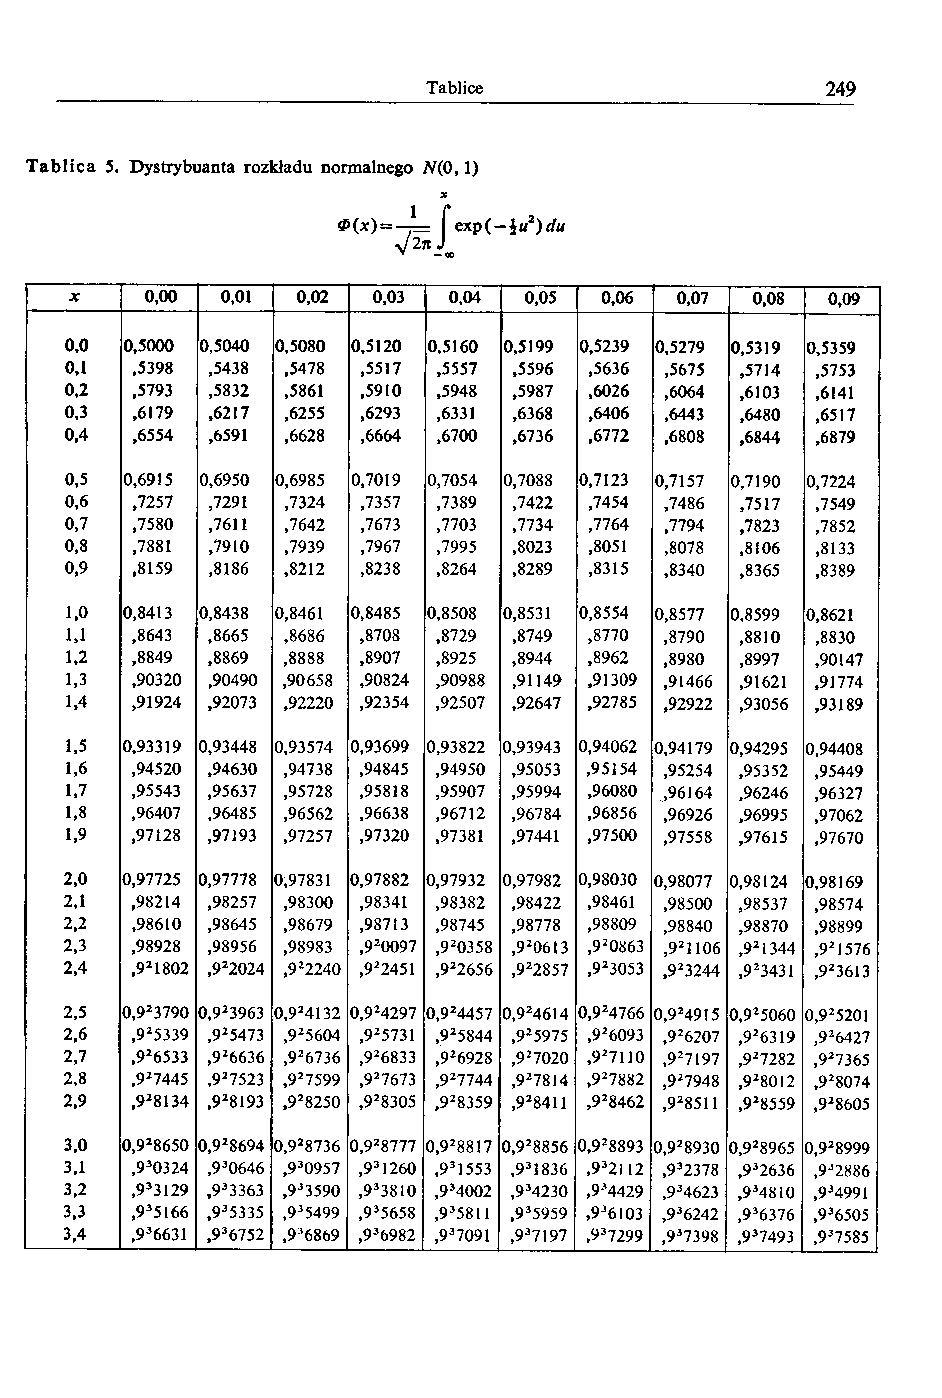
\includepdf[pages=-]{"pdf/DystNorm.pdf"}


\end{document}